\documentclass[a4paper, 12pt]{article}
\newcommand{\template}{../../Templates}
\usepackage{\template/package}
\usepackage[utf8]{inputenc}

\graphicspath{{../../Assets}}

\newcommand{\Titolo}{Analisi dei requisiti}
\newcommand{\Gruppo}{SWEnergy}
\newcommand{\Data}{17/11/2023}
\newcommand{\Mail}{\href{mailto:project.swenergy@gmail.com}{project.swenergy@gmail.com}}
\newcommand{\Versione}{0.1.0}
\newcommand{\Descrizione}{Documento che riporta un'analisi su casi d'uso e requisiti presenti nel capitolato.}
\newcommand{\Stato}{Non approvato / Approvato}
\newcommand{\Redattori}{Nome 1 \\ & Nome 2}
\newcommand{\Verificatori}{Nome 1 \\ & Nome 2}
\newcommand{\Approvatori}{Nome 1 \\ & Nome 2}
\newcommand{\Responsabile}{Nome 1}

\newcommand{\Titolo}{Valutazione capitolati}
\newcommand{\Gruppo}{SWEnergy}
\newcommand{\Data}{29/10/2023}
\newcommand{\Mail}{\href{mailto:project.swenergy@gmail.com}{project.swenergy@gmail.com}}
\newcommand{\Versione}{0.8.0}
\newcommand{\Descrizione}{
	L'analisi dei capitolati fa riferimento ai documenti presentati al link: \\
	\href{https://www.math.unipd.it/~tullio/IS-1/2023/Progetto/Capitolati.html}{Capitolati 2023}
}
\newcommand{\Stato}{Non approvato}
\newcommand{\Redattori}{
	Alessandro Tigani Sava \\ 
	& Carlo Rosso		\\
	& Davide Maffei		\\
	& Giacomo Gualato	\\
	& Matteo Bando 		\\ 
	& Niccolò Carlesso
}
\newcommand{\Verificatori}{Alessandro Tigani Sava \\ & Nome 2}
\newcommand{\Approvatori}{Nome 1}
\newcommand{\Responsabile}{}

\newcommand{\copertina}{    
	\begin{titlepage}
		\vspace*{-3.5cm}
    	\makebox[\textwidth]{
\includegraphics[width=\paperwidth]{img/header.png}}
		\begin{center}
			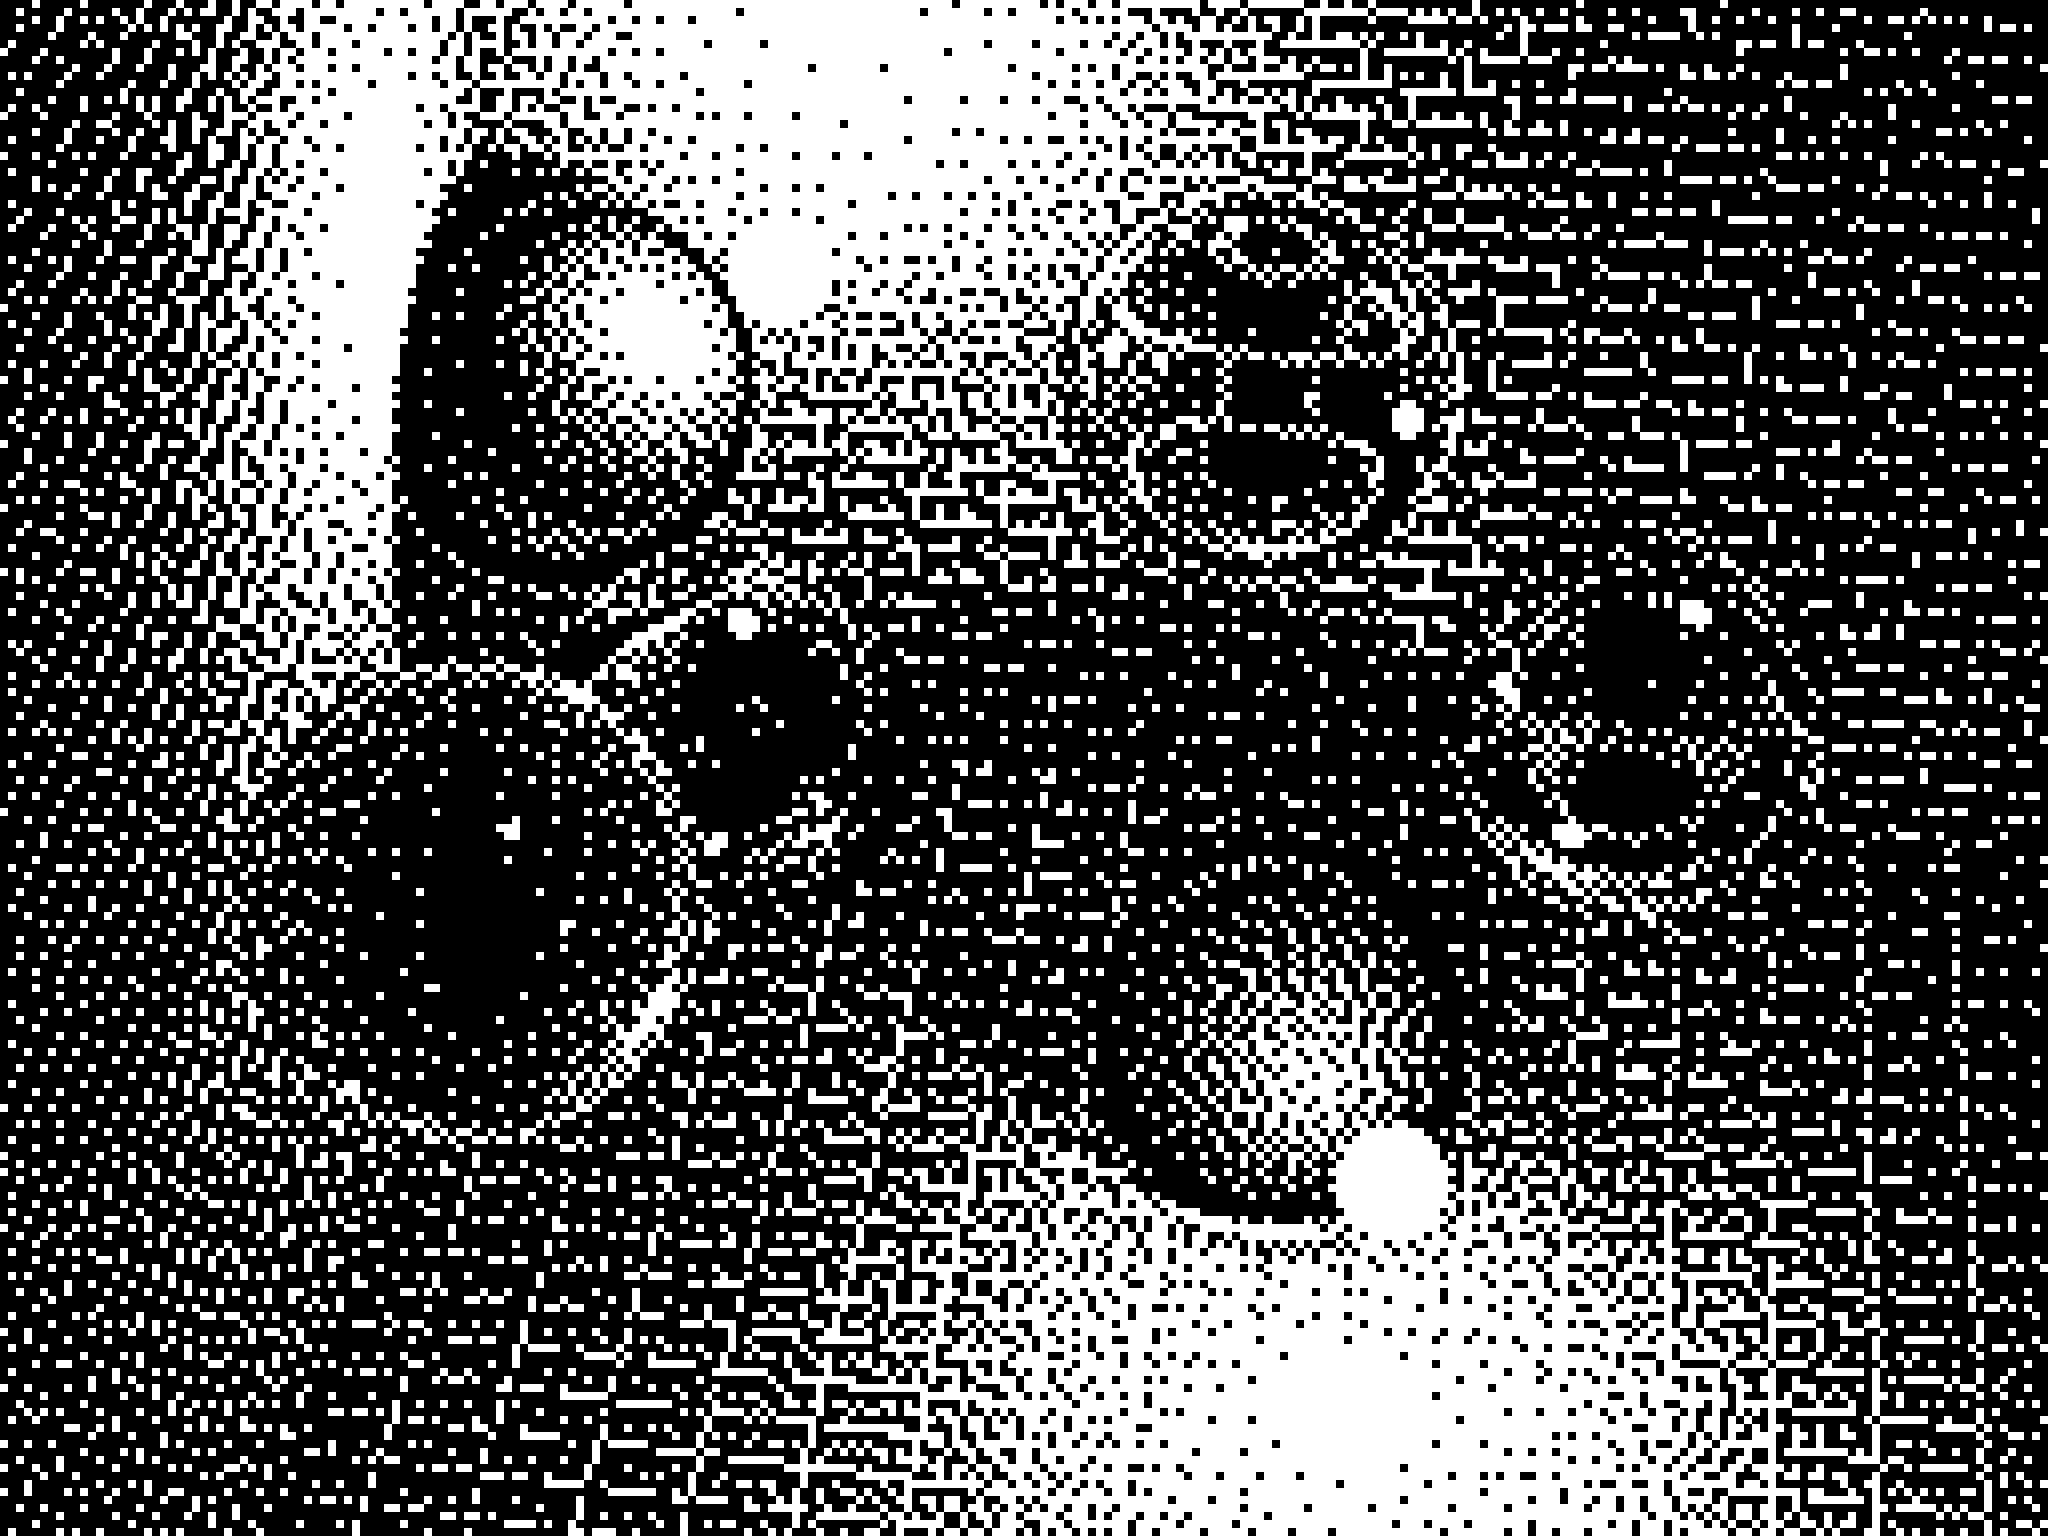
\includegraphics[width=1\textwidth]{img/logo}	\\
			\vspace{1cm}
			\Mail{}	\\
			\vspace{0.5cm}
			\textbf{\begin{LARGE} \Titolo \end{LARGE}}	\\
			\vspace{1cm}
			\textbf{Descrizione:} \Descrizione{} \\
			\vspace{1cm}
		\end{center}
		\begin{center}
			{
			\renewcommand{\arraystretch}{1.5}
			\begin{tabular}{ll}
				\textbf{Stato} 			& \Stato		\\ 
				\textbf{Data}			& \Data			\\
				\midrule
				\textbf{Redattori} 		& \Redattori 	\\  
				\textbf{Verificatori} 	& \Verificatori	\\
				\textbf{Approvatori} 	& \Approvatori	\\    
				\midrule
				\textbf{Versione}		& \Versione		\\
			   \end{tabular}
			}
		\end{center}
		%\vspace{3cm}
		%\begin{flushright}
		%	\begin{tabular}{ll}
		%		Il responsabile:	&  	\Responsabile	\\
		%							&					\\
		%							&	\underline{\hspace{3cm}} 	\\
		%	\end{tabular}
		%\end{flushright}
	\end{titlepage}
}

\fancypagestyle{plain}{
  	\fancyhf{}
  	\rhead{ 
\includegraphics[scale=0.05]{img/horizontal_logo.png}}
  	\lhead{\Titolo}
  	%\lfoot{\Titolo}
  	\rfoot{\thepage{}} 
  	\renewcommand{\headrulewidth}{0.2pt}
  	\renewcommand{\footrulewidth}{0.2pt}
}
\pagestyle{plain}



\begin{document}
% Cambio colore della prima pagina
%\newpagecolor{gray}            
%\afterpage{\restorepagecolor}

\copertina{}
\newpage
\section*{Registro delle modifiche}
 {
  \scriptsize
  \begin{tabular}{p{0.10\linewidth}p{0.10\linewidth}p{0.15\linewidth}p{0.15\linewidth}p{0.15\linewidth}p{0.19\linewidth}}
	  \textbf{Versione} & \textbf{Data} & \textbf{Redattore}     & \textbf{Verificatore} & \textbf{Approvatore} & \textbf{Descrizione}                                                                                                                     \\
	  \toprule
	  2.0.1             & 27/02/2024    & Davide Maffei          & Carlo Rosso           & /                    & Correzioni in seguito alla revisione RTB                                                                                                 \\
	  \hline
	  2.0.0             & 27/02/2024    & /                      & /                     & Niccolò Carlesso     & Approvazione finale del documento                                                                                                        \\
	  \hline
	  1.5.0             & 26/02/2024    & Alessandro Tigani Sava & Carlo Rosso           & /                    & Descrizione metriche di qualità                                                                                                          \\
	  \hline
	  1.4.1             & 14/02/2024    & Davide Maffei          & Giacomo Gualato       & /                    & Allineamento delle sezioni dei ruoli                                                                                                     \\
	  \hline
	  1.4.0             & 14/02/2024    & Davide Maffei          & Giacomo Gualato       & /                    & Creazione delle sezioni dei processi primari, di supporto e organizzativi                                                                \\
	  \hline
	  1.3.0             & 8/01/2024     & Carlo Rosso            & Niccolò Carlesso      & /                    & Correzione della sotto-sezione "Aggiornamento delle "Norme di Progetto"" e aggiunte le sotto-sezioni "Revisione del codice" e "Codifica" \\
	  \hline
	  1.2.0             & 31/12/2023    & Carlo Rosso            & Niccolò Carlesso      & /                    & Ristrutturazione del documento per ruolo, piuttosto che per argomento                                                                    \\
	  \hline
	  1.1.0             & 30/10/2023    & Carlo Rosso            & Giacomo Gualato       & /                    & Aggiornamento della sezione dedicata alla documentazione e aggiunta una sezione dedicata agli appunti                                    \\
	  \hline
	  1.0.0             & 30/10/2023    & /                      & /                     & Giacomo Gualato      & Approvazione finale del documento                                                                                                        \\
	  \hline
	  0.2.1             & 29/10/2023    & Alessandro Tigani Sava & Niccolò Carlesso      & /                    & Modifica procedure in sezione Approvazione di un documento                                                                               \\
	  \hline
	  0.2.0             & 24/10/2023    & Matteo Bando           & Niccolò Carlesso      & /                    & Redazione sezioni Versionamento, Verifica di un documento, Approvazione di un documento                                                  \\
	  \hline
	  0.1.0             & 23/10/2023    & Alessandro Tigani Sava & Matteo Bando          & /                    & Redazione sezioni Introduzione, Strumenti, Creazione e modifica di un documento, Ruoli, Registro delle modifiche                         \\
	  \hline
  \end{tabular}
 }

\newpage
\tableofcontents


\section{Introduzione}

Il presente documento, intitolato "Piano di Progetto", descrive e spiegare le
decisioni organizzative adottate dal gruppo SWEnergy per lo sviluppo del
progetto "\textit{Easy Meal}", proposto dall'azienda
\href{https://imolainformatica.it/}{Imola Informatica}. Il "Piano di Progetto" è
suddiviso nelle seguenti sezioni:

\begin{itemize}
	\item \textbf{Analisi dei rischi}: identifica i rischi individuati dal
	      gruppo e le strategie per mitigarli;

	\item \textbf{Modello di sviluppo}: descrive l'organizzazione temporale del
	      team di SWEnergy;

	\item \textbf{Pianificazione}: dettaglia la pianificazione del lavoro del
	      gruppo, incluse le attività, le risorse e i tempi necessari per lo
	      sviluppo del progetto;

	\item \textbf{Preventivo}: presenta il preventivo delle ore di lavoro e il
	      costo totale del progetto;

	\item \textbf{Consuntivo}: riporta le ore di lavoro e il costo effettivo del
	      progetto fino al momento della stesura del piano di progetto della
	      fase corrente: RTB.
\end{itemize}

\subsection{Scopo del documento}

Questo documento ha lo scopo di raccogliere in modo organico, coerente e
uniforme tutte le informazioni riguardanti la pianificazione del progetto, al
fine di fornire un riferimento per la gestione dello stesso. Al termine della
prima fase del progetto (RTB), verrà utilizzato per valutare l'andamento del
lavoro e per spiegare le decisioni adottate durante la pianificazione.

\subsection{Scopo del prodotto}

"\textit{Easy Meal}" è una web app progettata per gestire le prenotazioni
presso i ristoranti, sia dal lato dei clienti che dei ristoratori. Il prodotto
finale sarà composto da due parti:

\begin{itemize}
	\item \textbf{Cliente}: consente ai clienti di prenotare un tavolo presso un
	      ristorante, visualizzare il menù e effettuare un ordine;

	\item \textbf{Ristoratore}: consente ai ristoratori di gestire le
	      prenotazioni e gli ordini dei clienti, oltre a visualizzare la lista
	      degli ingredienti necessari per preparare i piatti ordinati.
\end{itemize}

\subsection{Glossario}

Al fine di evitare ambiguità linguistiche e garantire un'utilizzazione coerente
delle terminologie nei documenti, il gruppo ha redatto un documento interno
chiamato "Glossario". Questo documento definisce in modo chiaro e preciso i
termini che potrebbero generare ambiguità o incomprensione nel testo. I termini
presenti nel Glossario sono identificati da una 'G' (per esempio parola$_G$) a
pedice.

\subsection{Riferimenti}

\subsubsection{Normativi}
\begin{itemize}
	\item "\textit{Way of Working}";
	\item 	\href{https://www.math.unipd.it/~tullio/IS-1/2023/Progetto/C3.pdf}
	      {Documento del capitolato d'appalto C3 - \textit{Easy Meal}};
	\item \href{https://www.math.unipd.it/~tullio/IS-1/2023/Dispense/PD2.pdf}
	      {Regolamento del progetto};
\end{itemize}

\subsubsection{Informativi}

Slide dell'insegnamento di Ingegneria del Software:
\begin{itemize}
	\item \href{https://www.math.unipd.it/~tullio/IS-1/2023/Dispense/T3.pdf}
	      {Modelli di sviluppo del software};
	\item \href{https://www.math.unipd.it/~tullio/IS-1/2023/Dispense/T4.pdf}
	      {Gestione di progetto};
	\item \href{https://www.math.unipd.it/~tullio/IS-1/2023/Dispense/T5.pdf}
	      {Analisi dei requisiti};
\end{itemize}

\subsection{Scadenze}
Il \textit{team} di SWEnergy si impegna a rispettare le seguenti scadenze per il
completamento del progetto:
\begin{itemize}
	\item \textbf{Prima revisione (avanzamento RTB}: 21 dicembre 2023;
	\item \textbf{Seconda revisione (avanzamento PB)}: da definire;
	\item \textbf{Terza revisione (avanzamento CA)}: da definire;
\end{itemize}

\section{Descrizione del prodotto}
Il progetto mira a migliorare l'esperienza nei ristoranti sia per i clienti che per i ristoratori.
Si concentrerà sulle difficoltà legate alle prenotazioni e agli ordini, semplificando questi processi attraverso un'applicazione \textit{web} responsiva.
L'\textit{app} consentirà agli utenti di prenotare tavoli in modo intuitivo, personalizzare gli ordini in base alle proprie preferenze alimentari e favorire l'interazione tra clienti e personale del ristorante.
Inoltre, faciliterà la divisione del conto e promuoverà la scrittura di recensioni.

\subsection{Funzionalità}

\begin{itemize}
	\item \textbf{Registrazione di nuovi utenti:} Gli utenti possono creare un account per accedere a tutte le funzionalità dell'applicazione.
	\item \textbf{Prenotazione di un tavolo:} Gli utenti possono prenotare un tavolo in un ristorante in base alla disponibilità.
	\item \textbf{Ordinazione collaborativa dei pasti:} Gli utenti possono collaborare per ordinare i pasti, permettendo a ciascuno di aggiungere piatti al carrello.
	\item \textbf{Interazione con lo staff del ristorante:} Gli utenti possono comunicare con lo staff del ristorante per fare richieste speciali o per risolvere problemi.
	\item \textbf{Divisione del conto:} L'applicazione offre la possibilità di dividere il conto tra gli utenti in modo equo.
	\item \textbf{Consultazione delle prenotazioni da parte di un amministratore del ristorante:} Gli amministratori del ristorante possono consultare le prenotazioni per gestire la disponibilità dei tavoli.
	\item \textbf{Inserimento di \textit{feedback} e recensioni:} Gli utenti possono lasciare \textit{feedback} e recensioni sui ristoranti e sui piatti ordinati.
\end{itemize}

\subsection{Attori}
Gli attori che interagiscono con il sistema sono i seguenti:
% Servonno anche le immagini?
% Manca Utente generico
\begin{itemize}
	\item \textbf{Utente generico:} si tratta di un utente che non ha eseguito l'autenticazione
	\item \textbf{Utente base:} si tratta di un attore autenticato, rappresenta un possibile cliente di un ristorante
	\item \textbf{Utente ristoratore:} si tratta di un attore autenticato, rappresenta l'amministratore del ristorante
\end{itemize}

\subsection{Requisiti non funzionali}

\section{Casi d'uso}

Il gruppo di analisi ha identificato diversi casi d'uso nel capitolato d'appalto proposto, raggruppandoli in tipologie distinte. 
Le seguenti nomenclature vengono utilizzate per indicare i casi d'uso:

\begin{itemize}
	\item UCG : indica un caso d'uso strettamente legato all'Utente generico.
	\item UCA : indica un caso d'uso strettamente legato all'Utente autenticato.
	\item UCB : indica un caso d'uso strettamente legato all'Utente base.
	\item UCR : indica un caso d'uso strettamente legato all'Utente ristoratore.
	\item UCE : indica un caso d'uso strettamente legato ad un errore.
\end{itemize}

\subsection{Attori}

Gli attori identificati per il sistema e le relative dipendenze sono i seguenti:
\begin{itemize}
	\item \textbf{Utente generico}: è un utente che non ha effettuato l'accesso al
	      sistema. Può essere un utente non registrato o un utente registrato che non ha
	      ancora effettuato l'accesso;

	\item \textbf{Utente autenticato}: l'utente autenticato rappresenta un utente
	      base oppure un utente ristoratore che ha effettuato l'accesso al sistema.

	\item \textbf{Utente base}: l'utente base può compiere tutte le azioni
	      dell'Utente generico. Inoltre, può effettuare l'accesso al sistema e può
	      effettuare delle prenotazioni e attività correlate. L'utente base rappresenta
	      il cliente del ristorante;

	\item \textbf{Utente ristoratore}: l'utente ristoratore può compiere tutte le
	      azioni dell'Utente generico. Inoltre, può gestire il proprio ristorante e le
	      prenotazioni ad esso associate. L'utente ristoratore rappresenta il gestore del
	      ristorante;
\end{itemize}


\usecasegenerico{Effettua accesso}
\label{usecase:Effettua accesso}

\begin{itemize}
	\item \textbf{Descrizione:} Un Utente generico decide di effettuare l'accesso all'interno della \textit{web app}. Per effettuare tale
	operazione gli vengono presentate due opzioni:
	\begin{itemize}
		\item Accesso tramite inserimento di \textit{email} e \textit{password}.
		\item Accesso tramite un sistema di terze parti.
	\end{itemize}
	Nel caso in cui l'autenticazione fallisca, l'Utente generico deve inserire nuovamente le credenziali.

	\item \textbf{Attore principale:} Utente generico.
	\item \textbf{Attore secondario:} Sistema di autenticazione esterno.
	\item \textbf{Precondizioni:}
	      Un Utente generico è connesso al Sistema ed è in possesso di un \textit{account}.
	\item \textbf{Postcondizioni:}
	      L'Utente generico è stato identificato dal Sistema come uno solo dei seguenti:
	      \begin{itemize}
		      \item Utente ristoratore.
		      \item Utente base.
	      \end{itemize}
		  L'utente autenticato viene reindirizzato alla pagina \textit{Home} di pertinenza.

	\item \textbf{Scenario principale:}
	      \begin{enumerate}
		      \item L'Utente generico seleziona la tipologia di accesso: 

			  \begin{itemize}
				\item Accesso per terze parti (vedi \autoref{usecase:Accesso per terze parti}).
				\item Accesso tradizionale (vedi \autoref{usecase:Accesso tradizionale}).
			  \end{itemize}

		      \item Il Sistema verifica se l'Utente generico è un Utente ristoratore oppure Utente base;
		      \item L'Utente autenticato viene reindirizzato alla \textit{Home} impostata a seconda della tipologia di \textit{account}.		
	      \end{enumerate}
		
	\item \textbf{Scenario secondario:}
	\begin{itemize}
		\item \autoref{usecase:Accesso fallito} Accesso fallito:
		\begin{enumerate}
			\item L'autenticazione è fallita (vedi \autoref{usecase:Accesso fallito});
			\item L'Utente generico viene indirizzato nuovamente nella pagina di accesso;.
		\end{enumerate}	
	\end{itemize}

		

\end{itemize}

\subusecasegenerico{Accesso per terze parti}
\label{usecase:Accesso per terze parti}
\begin{itemize}

	\item \textbf{Attore principale:} Utente generico.
	\item \textbf{Attore secondario:} Sistema di autenticazione esterno.

	\item \textbf{Precondizioni:} Un Utente generico è connesso al Sistema ed è in possesso di un \textit{account}.

	\item \textbf{Postcondizioni:} Sono state verificate \textit{email} e \textit{password} dal Sistema di autenticazione esterno.

	\item \textbf{Scenario principale:}
	\begin{enumerate}
		\item Il Sistema reindirizza l'Utente generico alla pagina di accesso per terze parti;
		\item Il Sistema di autenticazione esterno verifica le credenziali;
		\item Il Sistema di autenticazione esterno invia al Sistema le informazioni dell'Utente generico;
		\item Il Sistema di autenticazione esterno reindirizza l'Utente generico alla pagina di accesso.
	\end{enumerate}
	
\end{itemize}

\subusecasegenerico{Accesso tradizionale}
\label{usecase:Accesso tradizionale}
\begin{itemize}

	\item \textbf{Attore principale:} Utente generico.

	\item \textbf{Precondizioni:} Un Utente generico è connesso al Sistema ed è in possesso di un \textit{account}.

	\item \textbf{Postcondizioni:} Sono state verificate \textit{email} e \textit{password}.

	\item \textbf{Scenario principale:}
	\begin{enumerate}
		\item L'Utente generico inserisce le credenziali del suo \textit{account}.
		\item Il Sistema verifica le credenziali.
	\end{enumerate}

\end{itemize}

\usecasebase{Prenotazione di un tavolo}
\label{usecase:Prenotazione di un tavolo}
\begin{itemize}
	\item \textbf{Attore principale:} Utente base.
	\item \textbf{Precondizioni:}
		\begin{itemize}
			\item Un Utente base ha effettuato l'accesso al Sistema (vedi \autoref{usecase:Effettua accesso});
			\item Un Utente base visualizza la pagina di dettaglio di un ristorante (\autoref{usecase:Visualizzazione di un ristorante});
		\end{itemize}
	\item \textbf{Postcondizioni:}
		\begin{itemize}
			\item L'Utente base ha confermato una prenotazione ed è tornato alla \textit{Home}.
		\end{itemize} 
	      
	\item \textbf{Scenario principale:}
	      \begin{enumerate}
		      \item L'Utente base compila una \textit{form} di prenotazione;
		      \item L'Utente base seleziona il giorno e l'ora;
		      \item L'Utente base seleziona il numero di persone;
		      \item L'Utente base inserisce eventuali necessità: particolare bisogno di seggiolini per bambini oppure se è presente un commensale con qualche disabilità o problemi di movimento;
		      \item L'Utente base inserisce lo username degli altri commensali che partecipano alla prenotazione (oppure la \textit{mail} se l'utente non è regisrato).
			  L'utente può anche decidere di non eseguire questo passaggio;
		      \item L'Utente base conferma la prenotazione.
		      \item Il Sistema registra la prenotazione.
		      \item Il Sistema crea un link condivisibile con il resto dei commensali(vedi \textit{extend:} \autoref{usecase:Condividi la prenotazione});
		      \item Il Sistema notifica la prenotazione all'Utente ristoratore (vedi \textit{extend:} \autoref{usecase:Notifica prenotazione}).
	      \end{enumerate}

	\item \textbf{Scenario secondario:}
	      \begin{itemize}
		      \item L'Utente base annulla la prenotazione (vedi
		            \autoref{usecase:Annullamento della prenotazione}).
		            \begin{enumerate}
			            \item L'Utente base annulla la prenotazione;
			            \item Il Sistema aggiorna la prenotazione.
			            \item Il Sistema notifica l'annullamento della prenotazione
			                  all'Utente ristoratore.
		            \end{enumerate}
	      \end{itemize}
\end{itemize}


\newpage
\usecasebase{Creazione dell'ordinazione collaborativa dei pasti}
\label{usecase:Creazione dell'ordinazione collaborativa dei pasti}

\begin{figure}[h]
	\centering
	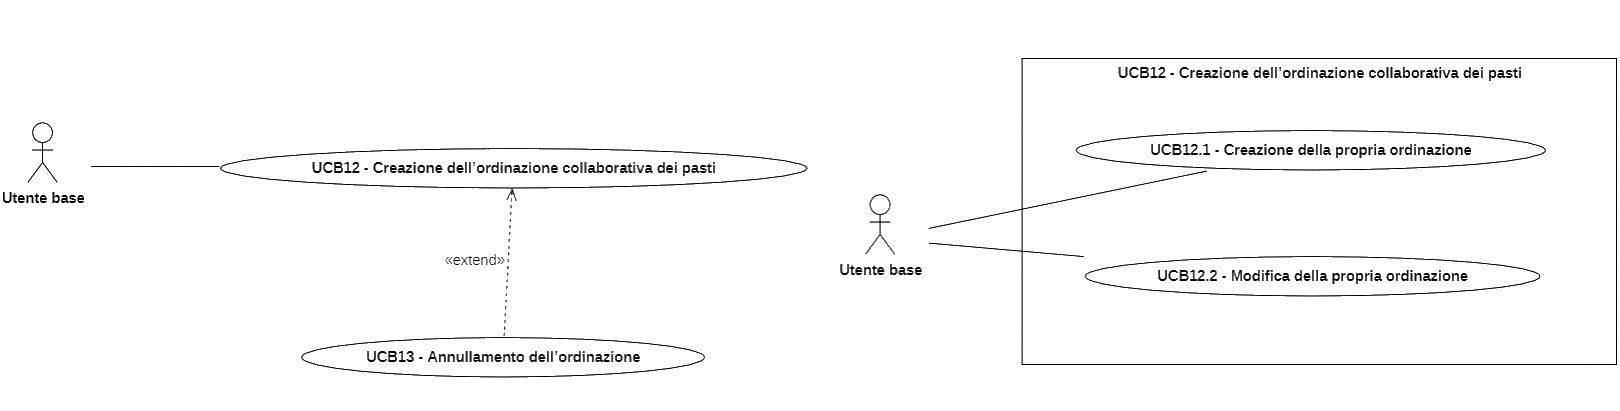
\includegraphics[width=0.9\textwidth]{./uml/UCB12-13.png} 
	\caption{Creazione dell'ordinazione collaborativa dei pasti}
	\label{fig:UCB12-13}
  \end{figure}

\begin{itemize}
	\item \textbf{Attore principale:} Utente base.

	\item \textbf{Precondizioni:}
	      \begin{itemize}
		      \item L'Utente base ha effettuato l'accesso al Sistema (vedi \autoref{usecase:Effettua accesso}).
		      \item L'Utente base ha effettuato una prenotazione (bedi \autoref{usecase:Prenotazione di un tavolo}).
		      \item L'Utente base sta visualizzando il riepilogo di una prenotazione (vedi \autoref{usecase:Visualizzazione del riepilogo prenotazione}) che si deve trovare nello stato: "Accettata"  (vedi \autoref{usecase:Accetta prenotazione}).
	      \end{itemize}

	\item \textbf{Postcondizione:} Un Utente base ha ordinato le pietanze per la prenotazione effettuata.

	\item \textbf{Scenario principale:}
	      \begin{enumerate}
		      \item L'Utente base visualizza le ordinazioni di tutti gli altri commensali collegati alla stessa prenotazione;
		      \item L'Utente base crea il proprio ordine$^G$ (vedi \autoref{usecase:Creazione della propria ordinazione});
		      \item L'Utente base modifica il proprio ordine (vedi \autoref{usecase:Modifica della propria ordinazione});

		      \item L'Utente base conferma il riepilogo dell'ordinazione;

		      \item Tutti gli Utenti base che partecipano all'ordinazione collaborativa dei pasti devono
		            confermare il riepilogo della loro ordinazione;
		      \item Il Sistema memorizza l'ordine.
	      \end{enumerate}

	\item \textbf{Scenario secondario:}
	      \begin{itemize}
		      \item L'Utente base annulla l'ordinazione (vedi
		            \autoref{usecase:Annullamento dell'ordinazione}).
		            \begin{enumerate}
			            \item L'Utente base annulla l'ordinazione;
			            \item Il Sistema aggiorna l'ordinazione.
		            \end{enumerate}
	      \end{itemize}
\end{itemize}


\subusecasebase{Creazione della propria ordinazione}
\label{usecase:Creazione della propria ordinazione}
\begin{itemize}
	\item \textbf{Attore principale:} Utente base.

	\item \textbf{Precondizione:} L'Utente base sta effettuando un ordinazione collaborativa dei pasti (vedi \autoref{usecase:Creazione dell'ordinazione collaborativa dei pasti});

	\item \textbf{Postcondizioni:}
	      \begin{itemize}
		      \item L'Utente base ha creato il proprio ordine.
		      \item Il Sistema aggiorna le informazioni inerenti al suo ordine.
	      \end{itemize}

	\item \textbf{Scenario principale:}
	      \begin{enumerate}
		      \item L'Utente base seleziona delle pietanze (vedi \autoref{usecase:Seleziona pietanza});
		      \item L'Utente base conferma il proprio ordine;
		      \item Il Sistema aggiorna il riepilogo dell'ordinazione.
	      \end{enumerate}
\end{itemize}


\subsubusecasebase{Seleziona pietanza}
\label{usecase:Seleziona pietanza}
\begin{itemize}
	\item \textbf{Attore principale:} Utente base.

	\item \textbf{Precondizione:} L'Utente base si trova nella sezione "Creazione della propria ordinazione" (vedi \autoref{usecase:Creazione della propria ordinazione}).

	\item \textbf{Postcondizione:} L'Utente base ha selezionato una pietanza.

	\item \textbf{Scenario principale:}
	      \begin{enumerate}
		      \item L'Utente base seleziona tra le lista delle pietanze una che vuole aggiungere al proprio ordine;
		      \item L'Utente base seleziona la quantità della pietanza;
		      \item L'Utente base conferma la sua selezione;
		      \item Il Sistema registra la sua selezione.
	      \end{enumerate}
\end{itemize}

\usecase{Interazione con il business}
\label{usecase:Interazione con il business}
\begin{itemize}
	\item \textbf{Attore principale:} Utente base.
	\item \textbf{Attori secondari:}
	      \begin{itemize}
		      \item Utente ristoratore;
		      \item Sistema.
	      \end{itemize}
	\item \textbf{Precondizioni:} L'Utente base è connesso al Sistema.
	\item \textbf{Postcondizioni:} L'Utente base ha interagito con il business.
	\item \textbf{Scenario principale:}
	      \begin{enumerate}
		      \item L'Utente base accetta i termini di utilizzo delle
		            conversazioni, se non l'ha già fatto;

		      \item L'Utente base visualizza un ristorante (vedi
		            \autoref{usecase:Visualizzazione di un ristorante});

		      \item L'Utente base accede alla sezione per \textit{chattare} con
		            l'Utente ristoratore;

		      \item L'Utente base invia un messaggio all'Utente ristoratore;

		      \item Il Sistema instaura una canale di comunicazione
		            crittografato tra l'Utente base e l'Utente ristoratore, se
		            non l'ha già fatto;

		      \item L'Utente ristoratore e l'Utente base comunicano tra di loro
		            fino a quando l'Utente base non termina la conversazione (vedi
		            \autoref{usecase:Visualizza la conversazione}, \autoref{usecase:Invia un
			            messaggio} %e \autoref{usecase:Elimina la conversazione}
		            ).
	      \end{enumerate}
\end{itemize}

\subusecase{Visualizza la conversazione}
\label{usecase:Visualizza la conversazione}
\begin{itemize}
	\item \textbf{Attore principale:} Utente autenticato$_1$.
	\item \textbf{Attori secondari:}
	      \begin{itemize}
		      \item Utente autenticato$_2$;
		      \item Sistema.
	      \end{itemize}
	\item \textbf{Precondizioni:} L'Utente autenticato$_1$ è connesso al
	      Sistema.
	\item \textbf{Postcondizioni:} L'Utente autenticato$_1$ visualizza la conversazione
	      con l'Utente autenticato$_2$.

	\item \textbf{Scenario principale:}
	      \begin{enumerate}
		      \item L'Utente autenticato$_1$ accede alla sezione delle conversazioni;
		      \item L'Utente autenticato$_1$ seleziona la conversazione con l'Utente
		            autenticato$_2$;
		      \item Il Sistema mostra i messaggi scambiati tra l'Utente
		            autenticato$_1$ e l'Utente autenticato$_2$.
	      \end{enumerate}
\end{itemize}

\subusecase{Invia un messaggio}
\label{usecase:Invia un messaggio}
\begin{itemize}
	\item \textbf{Attore principale:} Utente autenticato$_1$.
	\item \textbf{Attori secondari:}
	      \begin{itemize}
		      \item Utente autenticato$_2$;
		      \item Sistema.
	      \end{itemize}
	\item \textbf{Precondizioni:} L'Utente autenticato$_1$ è connesso al
	      Sistema e sta visualizzando la conversazione con l'Utente autenticato$_2$ (vedi
	      \autoref{usecase:Visualizza la conversazione}).

	\item \textbf{Postcondizioni:} L'Utente autenticato$_1$ ha inviato un
	      messaggio all'Utente autenticato$_2$.
	\item \textbf{Scenario principale:}
	      \begin{enumerate}
		      \item L'Utente autenticato$_1$ invia un messaggio all'Utente
		            autenticato$_2$;
		      \item Il Sistema memorizza il messaggio nel database;
		      \item Il Sistema invia una notifica all'Utente autenticato$_2$.
	      \end{enumerate}
\end{itemize}

%\subusecase{Elimina la conversazione}
%\label{usecase:Elimina la conversazione}
%\begin{itemize}
%\item \textbf{Attore principale:} Utente autenticato$_1$.
%\item \textbf{Attore secondario:} Nessuno.
%\item \textbf{Precondizioni:} L'Utente autenticato$_1$ è connesso al
%Sistema e sta visualizzando la conversazione con l'Utente autenticato$_2$ (vedi
%\autoref{usecase:Visualizza la conversazione}).
%
%\item \textbf{Postcondizioni:} L'Utente autenticato$_1$ ha eliminato la
%conversazione con l'Utente autenticato$_2$.
%\item \textbf{Scenario principale:}
%\begin{enumerate}
%	\item L'Utente autenticato$_1$ elimina la conversazione con l'Utente
%	      autenticato$_2$;
%	\item Il Sistema cancella il \textit{link} tra l'Utente autenticato$_1$ e
%	      l'Utente autenticato$_2$ nel database.
%\end{enumerate}

\usecasebase{Selezione della modalità di divisione del conto}
\label{usecase:Selezione della modalità di divisione del conto}

\begin{figure}[h]
	\centering
	
\includegraphics[width=0.9\textwidth]{./uml/UCB14.png} 
	\caption{Selezione della modalità di divisione del conto}
	\label{fig:UCB14}
  \end{figure}

\begin{itemize}
	\item \textbf{Attore principale:} Utente base.
	
	\item \textbf{Precondizione:}
	\begin{itemize}
		\item L'Utente base ha concluso l'ordinazione collaborativa dei pasti (vedi \autoref{usecase:Creazione dell'ordinazione collaborativa dei pasti}).
		\item L'Utente base visualizza il riepilogo di una prenotazione (vedi \autoref{usecase:Visualizzazione del riepilogo prenotazione}) il quale stato risulta \textit{In Corso}. 
	\end{itemize}

	\item \textbf{Postcondizione:}
	      L'Utente base ha selezionato la modalità di divisione del conto e lo ha diviso secondo le sue preferenze.
	\item \textbf{Scenario principale:}
	      \begin{enumerate}
		      \item L'Utente base seleziona la modalità di divisione del conto
		            tra quelle disponibili:
					\begin{itemize}
						\item \textbf{Divisione equa:} il conto viene diviso in parti
							  uguali tra tutti gli Utenti base che hanno condiviso la
							  prenotazione. L'Utente base può scegliere di pagare più di
							  una quota.
		  
						\item \textbf{Proporzionale:} l'Utente base seleziona i piatti che vuole
							  pagare.
					\end{itemize}

		      \item L'Utente base conferma la modalità di divisione del conto;

		      \item Il Sistema memorizza la modalità di divisione del conto.
	      \end{enumerate}

	\item \textbf{Scenario secondario:}
		  \begin{itemize}
			  \item \autoref{usecase:Visualizzazione errore divisione del conto già effettuata} Modalità di divisione del conto già effettuata:
				\begin{enumerate}
					\item L'Utente base seleziona la modalità di divisione del conto
						tra quelle disponibili;
	
					\item L'Utente base conferma la modalità di divisione del conto;
	
					\item Il Sistema mostra un messaggio di errore e spiega che la
						modalità di divisione del conto è già stata scelta.
				\end{enumerate}
		  \end{itemize}

\end{itemize}


\usecase{Consultazione di una prenotazione da parte del business}
\label{usecase:Consultazione delle prenotazioni da parte del business}
\begin{itemize}
	\item \textbf{Attore principale:} Utente ristoratore

	\item \textbf{Precondizioni:} L'Utente ristoratore ha effettuato l'accesso
	      al sistema.

	\item \textbf{Postcondizioni:}
	      L'Utente ristoratore visualizza i dettagli relativi ad una prenotazione.

	\item \textbf{Scenario principale:}
	      \begin{enumerate}
		      \item L'Utente ristoratore seleziona la funzionalità di
		            consultazione delle prenotazioni;

		      \item Il Sistema mostra la lista delle prenotazioni effettuate
		            dai clienti;

		      \item L'Utente ristoratore visualizza le prenotazioni
		            effettuate dai clienti, raggruppate per giorno in un
		            calendario.

		      \item L'Utente ristoratore seleziona una prenotazione;

		      \item Il Sistema mostra i dettagli relativi alla prenotazione
		            selezionata.
	      \end{enumerate}
\end{itemize}

\usecase{Notifica un feedback}
\label{usecase:Feedback automatico}
\begin{itemize}
	\item \textbf{Attore principale:} Sistema.

	\item \textbf{Autore secondario:} Utente base.

	\item \textbf{Precondizioni:}
	      L'Utente base si connette al sistema per la prima volta, dopo aver
	      completato un ordine.

	\item \textbf{Postcondizioni:}
	      L'Utente base ha ricevuto la notifica di inserimento del feedback.

	\item \textbf{Scenario principale:}
	      \begin{enumerate}
		      \item Il Sistema invia una notifica all'Utente base per
		            ricordargli di inserire un feedback;

		      \item L'Utente base riceve la notiva e decide se inserire un
		            feedback o meno (vedi \autoref{usecase:Inserimento di feedback e
			            recensioni});
	      \end{enumerate}
\end{itemize}

\usecase{Consulta lista degli ingredienti}
\label{usecase:Consulta lista degli ingredienti}
\begin{itemize}
	\item \textbf{Attore principale:} Utente ristoratore.

	\item \textbf{Attore secondario:} Sistema.

	\item \textbf{Precondizioni:}
	      L'Utente ristoratore ha effettuato l'accesso al sistema.

	\item \textbf{Postcondizioni:}
	      L'Utente ristoratore ha visualizzato la lista degli ingredienti.

	\item \textbf{Scenario principale:}
	      \begin{enumerate}
		      \item L'Utente ristoratore seleziona la funzionalità di
		            visualizzazione della lista degli ingredienti.

		      \item Il Sistema mostra la lista degli ingredienti;

		      \item L'Utente ristoratore applica un filtro temporale alla lista
		            degli ingredienti;

		      \item Il Sistema mostra la lista degli ingredienti
		            relativi all'arco temporale di interesse;

		      \item L'Utente ristoratore può esportare la lista degli
		            ingredienti.
	      \end{enumerate}

	\item \textbf{Descrizione:}
	      Il filtro temporale è espresso in termini di data di scadenza da oggi.
	      Probabilmente l'esportazione della lista degli ingredienti sarà
	      effettuata in formato \texttt{.csv}.
\end{itemize}



\newpage
\usecaseautenticato{Effettua \textit{Logout}}
\label{usecase:Effettua Logout}

\begin{figure}[h]
	\centering
	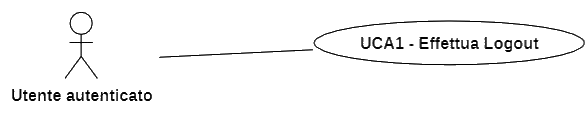
\includegraphics[width=0.8\textwidth]{./uml/UCA1.png} 
	\caption{Effettua \textit{Logout}}
	\label{fig:UCA1}
  \end{figure}

\begin{itemize}
	\item \textbf{Attore principale:} Utente autenticato.

	\item \textbf{Precondizione:} L'Utente ha eseguito correttamente l'accesso al Sistema come Utente base o Utente ristoratore(vedi \autoref{usecase:Effettua accesso}).

	\item \textbf{Postcondizione:} L'utente esegue con successo il \textit{logout}.

	\item \textbf{Scenario principale:}
	      \begin{enumerate}
		      \item L'Utente autenticato seleziona nell'\textit{header} della pagina la voce "\textit{Logout}".
		      \item L'Utente autenticato avvia la procedura di \textit{logout}.
              \item Il Sistema disconnette l'utente dal suo \textit{account} e lo reindirizza alla \textit{Home} del sito, identificandolo come Utente generico.
	      \end{enumerate}
\end{itemize}

\usecasegenerico{Visualizzazione ristorante}  
\label{usecase:Visualizzazione di un ristorante}
\begin{itemize}
	\item \textbf{Attore principale:} Utente generico.


	\item \textbf{Precondizioni:}
	\begin{itemize}
        \item L'utente è connesso al Sistema.
        \item L'utente ha selezionato un ristorante dalla lista di ristoranti proposta (vedi \autoref{usecase:Consultazione elenco ristoranti}).
    \end{itemize}

	\item \textbf{Postcondizione:} L'utente accede alle informazioni dettagliate del ristorante.

	\item \textbf{Scenario principale:}
		\begin{enumerate}
		    \item L'Utente seleziona il ristorante desiderato per visualizzarne i dettagli.
		    \item Il Sistema mostra le seguenti informazioni del ristorante:
		    \begin{itemize}
				\item \textbf{Nome:} denominazione del ristorante.
				\item \textbf{Descrizione:} una breve descrizione del ristorante.
				\item \textbf{Orario:} giorni della settimanana e fascia oraria in cui il ristorante è aperto.
				\item \textbf{Indirizzo:} ubicazione fisica del ristorante.
				\item \textbf{Recapiti:} numeri di telefono, indirizzo \textit{e-mail} o altri metodi di contatto escludendo l'utilizzo della \textit{chat}.
				\item \textbf{Prezzo:} fascia di prezzo del ristorante.
				\item \textbf{Voto:} media delle valutazioni del ristorante.
				\item \textbf{Cucina:} tipologia delle pietanze servite dal ristorante.
				\item \textbf{Menù:} elenco dei piatti offerti dal ristorante.
				\item \textbf{\textit{Link}:} collegamento ad un eventuale sito \textit{web} del ristorante. 
			\end{itemize}
	    \end{enumerate}

\end{itemize}
\usecase{Visualizzazione del riepilogo}
\label{usecase:Visualizzazione del riepilogo}
\begin{itemize}
	\item \textbf{Attore principale:} Utente base.

	\item \textbf{Attore secondario:} Sistema.

	\item \textbf{Precondizioni:}
	      Un Utente base ha effettuato l'accesso al Sistema ed è associato ad una
	      prenotazione (vedi \autoref{usecase:Prenotazione di un tavolo},
	      \autoref{usecase:Accedi alla prenotazione}).

	\item \textbf{Postcondizioni:}
	      L'Utente base visualizza il riepilogo della prenotazione.

	\item \textbf{Scenario principale:}
	      \begin{enumerate}
		      \item L'Utente base accede alla sezione delle prenotazioni;
		      \item L'Utente base seleziona una prenotazione;
		      \item Il Sistema mostra il riepilogo della prenotazione.
	      \end{enumerate}
\end{itemize}

\usecasebase{Condividi la prenotazione}
\label{usecase:Condividi la prenotazione}
\begin{itemize}
	\item \textbf{Attore principale:} Utente base.

	\item \textbf{Precondizioni:}
	\begin{itemize}
		\item L'Utente base ha effettuato al Sistema (vedi \autoref{usecase:Effettua accesso}).
		\item L'Utente base sta visualizzando il riepilogo di una prenotazione (vedi \autoref{usecase:Visualizzazione del riepilogo prenotazione}).
	\end{itemize}

	\item \textbf{Postcondizione:}
	      L'Utente base ha copiato il \textit{link} della prenotazione e lo ha condiviso agli altri commensali.

	\item \textbf{Scenario principale:}
	      \begin{enumerate}
		      \item L'Utente base seleziona l'opzione per condividere la prenotazione;
		      \item Il Sistema mostra il \textit{link} della prenotazione;
		      \item L'Utente base copia il \textit{link} della prenotazione;
		      \item L'Utente base invia il \textit{link} agli altri utenti.
	      \end{enumerate}
\end{itemize}
\usecasebase{Accedi alla prenotazione}
\label{usecase:Accedi alla prenotazione}
\begin{itemize}
	\item \textbf{Attore principale:} Utente base.

	\item \textbf{Precondizione:} 
	\begin{itemize}
		\item L'Utente base è connesso al Sistema (vedi \autoref{usecase:Effettua accesso});
		\item L'Utente base ha ricevuto il link di invito ad una prenotazione (vedi \autoref{usecase:Condividi la prenotazione})
	\end{itemize}
		

	\item \textbf{Postcondizione:} L'Utente base è collegato ad una prenotazione.

	\item \textbf{Scenario principale:}
	      \begin{enumerate}
		      \item L'Utente base ha ricevuto il link di invito ad una prenotazione da parte di un altro utente;
		      \item L'Utente base accetta l'invito;
		      \item L'Utente base è ora collegato ad una prenotazione;
	      \end{enumerate}

	\item \textbf{Scenario secondario:}
		  \begin{itemize}
			  \item \autoref{usecase:Accesso prenotazione fallito} Accesso prenotazione fallito:
			  \begin{enumerate}
				  \item L'autenticazione è fallita (vedi \autoref{usecase:Accesso prenotazione fallito});
				  \item L'Utente generico viene indirizzato nuovamente nella pagina di accesso; 
			  \end{enumerate}	
		  \end{itemize}
\end{itemize}

\usecase{Errore utente ristoratore}
\label{usecase:Errore utente ristoratore}
\begin{itemize}
	\item \textbf{Attore principale:} Utente esterno.
	\item \textbf{Attore secondario:} Sistema.
	\item \textbf{Precondizione:} L'Utente esterno sta effettuando l'accesso al
	      Sistema.
	\item \textbf{Postcondizione:} L'Utente esterno ha ricevuto un messaggio di errore.
	\item \textbf{Scenario principale:}
	      \begin{enumerate}
		      \item L'utente esterno effettua l'accesso al Sistema (vedi \autoref{usecase:Effettua accesso});
		      \item Il Sistema rileva che l'Utente esterno è un Utente ristoratore;
		      \item Il Sistema mostra un messaggio di errore.
	      \end{enumerate}
\end{itemize}

\usecasebase{Inserimento di feedback e recensioni}
\label{usecase:Inserimento di feedback e recensioni}
\begin{itemize}
	\item \textbf{Attore principale:} Utente base.

	\item \textbf{Precondizione:} L'Utente base ha completato un ordine e lo ha pagato (vedi \autoref{usecase:Pagamento del conto}).

	\item \textbf{Postcondizione:} L'Utente base ha lasciato un \textit{feedback} o una recensione.

	\item \textbf{Scenario principale:}
	      \begin{enumerate}
		      \item L'Utente base seleziona la prenotazione per la quale vuole
		            lasciare un \textit{feedback} o una recensione (vedi
		            \autoref{usecase:Visualizzazione del riepilogo prenotazione});

		      \item L'Utente base compila il \textit{form} del \textit{feedback} del ristorante;

		      \item L'Utente base conferma il \textit{feedback};

		      \item Il Sistema registra il \textit{feedback} o la recensione;

		      \item Il Sistema aggiorna la media dei punteggi del ristorante;

		      \item Il Sistema invia una notifica al ristoratore per avvisarlo
		            dell'inserimento di un nuovo \textit{feedback} o di una nuova
		            recensione (vedi \autoref{usecase:Notifica di inserimento feedback}).
	      \end{enumerate}
\end{itemize}

\usecase{Analisi dei dati}
\label{usecase:Analisi dei dati}
\begin{itemize}
	\item \textbf{Attore principale:} Utente ristoratore.

	\item \textbf{Attore secondario:} Sistema.

	\item \textbf{Precondizioni:}
	      L'utente ristoratore è connesso al Sistema.

	\item \textbf{Postcondizioni:}
	      L'utente ristoratore visualizza le statistiche relative al proprio
	      ristorante.

	\item \textbf{Scenario principale:}
	      \begin{enumerate}
		      \item L'utente ristoratore accede alla sezione di analisi dei
		            dati;

		      \item Il sistema mostra le statistiche relative al ristorante
		            dell'utente ristoratore;

		      \item L'utente ristoratore filtra le statistiche (per esempio
		            per periodo);

		      \item Il sistema mostra le statistiche filtrate.
	      \end{enumerate}
\end{itemize}


\usecase{Visualizzazione delle liste di ingredienti da parte del business}
\label{usecase:Visualizzazione delle lista ingredienti}
\begin{itemize}
	\item \textbf{Attore principale:} Utente ristoratore
	
	\item \textbf{Attore secondario:} Sistema

	\item \textbf{Precondizioni:} L'Utente ristoratore ha effettuato l'accesso
	      al sistema.

	\item \textbf{Postcondizioni:}
	      L'Utente ristoratore visualizza le lista di ingredienti che ha creato.

	\item \textbf{Scenario principale:}
	      \begin{enumerate}
		      \item L'Utente ristoratore seleziona la funzionalità di
		            visualizzazione delle liste di ingredienti;

		      \item Il Sistema permette di visualizzare il nome della lista di ingredienti 
			  indicando anche il relativo ristorante a cui si riferisce.

			  \item L'Utente ristoratore può selezionare una di queste liste per scegliere se 
			  modificarla o eliminarla.
			  Inoltre può accedere alla funzionalità di creazione di una nuova lista di ingredienti.
	      \end{enumerate}
\end{itemize}

\usecase{Creazione di una lista di ingredienti da parte del business}
\label{usecase:Creazione di una lista ingredienti}
\begin{itemize}
	\item \textbf{Attore principale:} Utente ristoratore

	\item \textbf{Attore secondario:} Sistema

	\item \textbf{Precondizioni:} L'Utente ristoratore ha effettuato l'accesso
	      alla funzionalità di visualizzazione lista ingredienti 
		  ((vedi \autoref{usecase:Visualizzazione delle lista ingredienti}).)

	\item \textbf{Postcondizioni:}
	      L'Utente ristoratore ha creato una lista di ingredienti disponibili.

	\item \textbf{Scenario principale:}
	      \begin{enumerate}
		      \item L'Utente ristoratore seleziona la funzionalità di
		            creazione di una lista di ingredienti e associarla ad un ristorante;

		      \item Il Sistema attraverso un \textit{form} permette di inserire i vari ingredienti utilizzati dal ristorante;
					Si possono inserire varie informazioni, come il nome dell'ingrediente, la disponibilità, il prezzo (\SI{}{\euro\per\kilo\gram}) e a che pietanze assegnarle.
	      \end{enumerate}
\end{itemize}

\usecase{Modifica di una lista di ingredienti}
\label{usecase:Modifica di una lista ingredienti}
\begin{itemize}
	\item \textbf{Attore principale:} Utente ristoratore
	
	\item \textbf{Attore secondario:} Sistema

	\item \textbf{Precondizioni:} L'Utente ristoratore ha effettuato l'accesso
	alla funzionalità di visualizzazione lista ingredienti e ha selezionato una lista ingredienti.
	((vedi \autoref{usecase:Visualizzazione delle lista ingredienti}).)

	\item \textbf{Postcondizioni:}
	      L'Utente ristoratore ha modificato la lista di ingredienti selezionata.

	\item \textbf{Scenario principale:}
	      \begin{enumerate}
		      \item L'Utente ristoratore seleziona la funzionalità di
		            modifica della lista di ingredienti selezionata;

		      \item Il Sistema attraverso un \textit{form} permette di visualizzare e modificare i vari valori inseriti in precedenza.
					Inoltre da l'opportunità di aggiungere un ingrediente, modificarlo o eliminarlo;
				
			  \item Il Sistema salva le modifiche e aggiorna la lista di ingredienti;
			  
			  \item Il Sistema riporta l'Utente ristorante alla \textit{Visualizzazione delle liste ingredienti}.
	      \end{enumerate}
\end{itemize}

\usecase{Eliminazione di una lista degli ingredienti}
\label{usecase:Elimina una lista degli ingredienti}
\begin{itemize}
	\item \textbf{Attore principale:} Utente ristoratore
	
	\item \textbf{Attore secondario:} Sistema

	\item \textbf{Precondizioni:} L'Utente ristoratore ha effettuato l'accesso
	alla funzionalità di visualizzazione lista ingredienti.
	((vedi \autoref{usecase:Visualizzazione delle lista ingredienti}).)

	\item \textbf{Postcondizioni:}
	      L'Utente ristoratore ha eliminato la lista di ingredienti selezionata.

	\item \textbf{Scenario principale:}
	      \begin{enumerate}
		      \item L'Utente ristoratore seleziona la funzionalità di
		            eliminazione della lista di ingredienti selezionata;

		      \item Il Sistema richiede conferma all'utente ristorante;
				
			  \item Il Sistema salva le modifiche dopo la conferma dell'utente ristorante;
			  
			  \item Il Sistema riporta l'Utente ristorante alla \textit{Visualizzazione delle liste ingredienti}.
	      \end{enumerate}
\end{itemize}


\usecase{Visualizzazione dello stato di un ordine}
\label{usecase:Visualizzazione dello stato di un ordine}
\begin{itemize}
	\item \textbf{Attore principale:} Utente autenticato.

	\item \textbf{Attore secondario:} Sistema.

	\item \textbf{Precondizioni:}
	      Un Utente autenticato ha effettuato e confermato una prenotazione e si trova presso il ristorante.

	\item \textbf{Postcondizioni:}
	      L'Utente base visualizza lo stato dell'ordine.

	\item \textbf{Scenario principale:}
	      \begin{enumerate}
		      \item L'Utente autenticato seleziona una prenotazione confermata;
		      \item Il Sistema mostra le varie pietanze ordinate e il loro stato 
			  (ancora da preparare, in preparazione, in consegna, consegnato) 
			  e il relativo tempo di attesa.
	      \end{enumerate}
\end{itemize}

\usecase{Sistema di filtraggio della lista dei ristoranti}
\label{usecase:Sistema di filtraggio della lista dei ristoranti}
\begin{itemize}
	\item \textbf{Attore principale:} Utente generico.

	\item \textbf{Attori secondario:} Sistema.

	\item \textbf{Precondizioni:}
	      Un Utente generico è connesso al Sistema.

	\item \textbf{Postcondizioni:}
	      L'Utente generico visualizza una lista dei ristoranti che soddisfa i filtri inseriti dall'Utente generico..

	\item \textbf{Scenario principale:}
	      \begin{enumerate}
			  \item Il sistema richiede il tracciamento GPS all'Utente generico per filtrare in base alla posizione più vicina.
		      \item L'Utente generico inserisce i parametri di ricerca, come il prezzo, tipo di cucina, posizione, popolarità, orario, ecc...;
		      \item L'Utente generico conferma la ricerca.
		      \item Il Sistema mostra i risultati della ricerca.
	      \end{enumerate}
\end{itemize}



\section{\textit{Technology baseline}}
 % diapositiva 11 di T5
% https://www.math.unipd.it/~tullio/IS-1/2023/Dispense/T5.pdf

\section{Requisiti}
Questa sezione fornisce un elenco dei requisiti minimi indispensabili per l'esecuzione dell'applicazione, illustrando le caratteristiche necessarie per configurare 
correttamente l'ambiente di sviluppo del progetto.

\subsection{Requisiti di sistema}
Affinché l'installazione e l'avvio del prodotto avvengano senza problemi e per garantire un'esperienza completa e soddisfacente nell'utilizzo 
dell'applicazione, è essenziale installare i seguenti \textit{software}.

\begin{longtable}{|c|c|c|}
	\hline
	\textbf{Componente}       & \textbf{ Versione}   & \textbf{ Riferimenti per il download} \\
	\hline
     Node.js             & $ \geq  20.x.x$            &\href{https://nodejs.org/en/}{https://nodejs.org/en/}        \\
    \hline
     npm                & $ \geq 9.x.x$            &Integrato con il download di Node.js        \\
    \hline

    \caption{Tabella dei requisiti di sistema.}
\end{longtable}


\subsection{Requisiti \textit{software}}
L'applicazione è stata testata e confermata come utilizzabile sui principali \textit{browser}, per i quali sono specificate le versioni iniziali che hanno costituito 
il punto di partenza per lo sviluppo del progetto. Durante lo sviluppo, si è considerato incrementalmente l'aggiornamento alle versioni più recenti dei singoli \textit{browser}.

\begin{longtable}{|c|c|c|}
	\hline
	\textbf{Browser}       & \textbf{ Versione}    \\
	\hline
    Google Chrome             & 123                    \\
    \hline
    Arc                       & 1.26                    \\
    \hline
    Opera GX                       & 124                    \\
    \hline
    Safari                        & 17.3                    \\
    \hline
    Microsfot Edge                 & 123                      \\
    \hline

    \caption{Tabella dei requisiti \textit{software}.}
\end{longtable}


\subsection{Requisiti \textit{hardware}}
Poiché l'applicazione funziona su un \textit{browser}, non ci sono requisiti specifici definiti dal proponente, dal capitolato o dal progetto stesso. 
Quindi, i seguenti requisiti sono considerati solo come linee guida generali per l'esecuzione del prodotto creato.

\begin{longtable}{|l|p{0.8\textwidth}|}
	\hline
	\textbf{Componente}       & \textbf{ Requisito minimo}   \\
	\hline
     Processore             &  Processore a 64 bit Quad-Core 3,2 GHz      \\
    \hline
     Memoria RAM            &  4GB DDR4       \\
    \hline
    Spazio su disco         & $ \geq  126 GB$         \\
    \hline
    Connessione Internet         & Connessione \textit{Internet} stabile e veloce, in grado di supportare le esigenze di traffico dell'applicazione         \\
    \hline

    \caption{Tabella dei requisiti \textit{hardware}.}
\end{longtable}

\end{document}
